%
% sdd.tex contains the Software/Database Design Document for the
%     Software Development Folder for the eCommerce CMS project for:
% CMSI 402
% Loyola Marymount University
%
% By Andrew Won
%

% ~~~~~~~~~~~~~~~~~~~~~~~~~~~~~~~~~~~~~~~~~~~~~~~~~~~~~~~~~~~~~~~~~~~~~~~~~~~~~
%  Revision History:
%  -----------------
%
%   Ver      Date      Modified by:  Description of change/modification
%  -----  -----------  ------------  ------------------------------------------
%  1.0.0  19-Mar-2013  A. Won        Initial version/release
%
% ~~~~~~~~~~~~~~~~~~~~~~~~~~~~~~~~~~~~~~~~~~~~~~~~~~~~~~~~~~~~~~~~~~~~~~~~~~~~~

\documentclass{article}
\usepackage{doc}
\usepackage[margin=1in]{geometry}
\usepackage{amsmath}
\usepackage{multirow}
\usepackage{graphicx}
\usepackage{float}
\geometry{letterpaper}

\title{eCommerce CMS Software/Database Design Document}
\author{Andrew Won}
\date{March 19, 2013}

\newcommand{\br}{\vspace{2mm}}

\begin{document}

\maketitle
\tableofcontents
\listoftables
\listoffigures

\pagebreak
\setcounter{section}{5}
\section{Software/Database Design Document}

\subsection{Introduction}

This document presents the architecture and detailed design for the eCommerce CMS
software for the CMSI 402 project at Loyola Marymount University.  eCommerce CMS
is a software solution for small business customers looking for
an initial online presence.  The eCommerce CMS application will offer both a
web service for HTTP requests and sets of internet-accessible web pages served
by that web service.

The eCommerce CMS application will offer a Java-based web service which will
allow for HTTP requests to qualified users.  The Java-based service will also
serve two sets of front-end web pages.  Through the first set, small business
users of the application can implement and manage an online business management
and sales solution. Through the second set, customers of the small business will
be able to interact with the small business either through making purchases on
an eCommerce web site or through committing information required for generation
of a proposal.

\subsubsection{System Objectives}

The objective of this application is to provide a new content management
system with customizable saleable inventory and customer user interfaces for
beginning, small-business eCommerce users.  Customers will be able to purchase
products and various reports and proposals will
be able to be generated from a single, easy to customize interface.  The
small business users of the application will be able to implement and manage
an online business management and sales solution.  In
addition, a secondary objective of this application is to deliver a high degree
of customizability requiring relatively low expertise in use of internet
technologies.

\subsubsection{Hardware, Software, and Human Interfaces}
\label{hshi}

\begin{enumerate}
    \item[~\ref{hshi}.1 ] \emph{HTTP Requests}\br\\
        HTTP requests are used by front-end pages to interface with all
        components in the back-end, see table~\ref{software-hierarchy} for a
        list of these components.  The HTTP requests are handled using the
        following third-party libraries:
        \begin{enumerate}
            \item JAX-RS
                Java API that supports web service endpoints according to the
                Representational State Transfer (REST) architecture.  Also known
                as ``Java API for RESTful Web Services.''
            \item Jersey
                JAX-RS implementation.
            \item JAXB
                Java architecture for XML Binding.
            \item Jackson
                Java library for processing the JSON data format.
        \end{enumerate}
    \item[~\ref{hshi}.2 ] \emph{Keyboard}\br\\
        A keyboard is used to interface with the user and customer front-ends,
        see table~\ref{software-hierarchy} for a list of these components.  Keyboard
        entries primarily allow customers and users to provide textual data,
        primarily through form fields.
    \item[~\ref{hshi}.3 ] \emph{Pointer Device}\br\\
        A pointer device is used to interface with the user and customer
        front-ends, see table~\ref{software-hierarchy} for a list of these
        components.  The pointer device, such as a mouse, is the primary
        way of navigating the user and customer front-ends, which are built
        primarily using the Menus, Forms, and Dialogs interface style.
    \item[~\ref{hshi}.4 ] \emph{Network Interface Controller}\br\\
        A Network Interface Controller is used to interface with the user and
        customer front-ends by facilitating a connection for the customer or
        user to a webpage hosted on a server hosting the application, see
        table~\ref{software-hierarchy} for a list of these components.  Because
        the service is accessed through HTTP requests and the webpages are
        served through web servers, a network connection is required for all
        interaction with the application.
\end{enumerate}

% If you use HTTP or SSL for communication through a browser, put that in.
% If third party libraries are
% used, list each of them in a separately numbered paragraph which describes
% the purpose of use, the version used, and the portions of your project which
% will interface with them.

% Describe the user interface, GUI, or TUI which you
% will implement, and include a screen shot or simulated drawing of its
% appearance. Make sure to include the hardware interfaces, such as networking,
% mouse, keyboard, and so on. Use paragraph numbers like "6.1.2.1" and "6.1.2.2".

\pagebreak
\subsection{Architectural Design}

% The architectural design of a software system is one of the most critical
% aspects of a successful system. A good design generally takes considerable
% foresight and a lot of trial and error through iterations. The length of this
% section of the document can be fairly short, but the thought that goes into
% it should be substantial.

% The architectural design is the first step towards an implementation.
% The requirements specification has previously identified the functions the
% customer requires which the programmer will be implementing. The
% architectural design suggests an implementation of those functions. This does
% not mean the architectural design will simply be a module for each of the
% functions described in the requirements specification.

% One of the most important characteristics of a good designer is that s/he
% be able to spot awkwardness in a design. This means that you must look at the
% design and attempt to figure if it works from the perspective of, "Now if I
% had to implement this module, could I do it reasonably?" In general, you are
% looking for the problem, "I need to compute the sine of X, but I haven't been
% told X and I can't find it out." Another common problem in design is a lack
% of independence between the modules. This is known as coupling, and has the
% related term cohesion. Refer to sections 7.2 and 7.3 of your textbook for
% more definitive definitions of these terms, but the gist is you want a
% software design which has loose coupling and relatively tight cohesion.
% Design awkwardness will cause a lot of confusion on a group project, because
% different people will be working on each module; it can also be a source of
% confusion to single-developer projects.

% This section of your SDF should present the overall design of the system.
% Partition the system into logical sets of class definitions. These classes
% should be based on their overall functionality within the entire application.
% For example, you might want to decompose the system into State Control, User
% Interface Control, and Computer Player subsystems. The goal of this section
% is to give some conceptual organization to the detailed descriptions that are
% to follow.

\subsubsection{Major Software Components}
\label{msc}

\begin{enumerate}
    \item[~\ref{msc}.1 ] \emph{Back-End: HTTP Resources}\br\\
        eCommerce CMS accepts HTTP requests through URI endpoints as outlined
        later in this document.  A user or web browser can initiate the HTTP
        request to communicate with the web service.
    \item[~\ref{msc}.2 ] \emph{Back-End: Persistent Data Store}\br\\
        eCommerce CMS offers a persistent data store through a database.  The
        persistent data store is generated by Hibernate, a Java Object/Relational
        Mapping tool, and stored in an instance of PostgreSQL, a relational
        database.

        The persistent data store maintains saleable items and services, templates
        for generating documents, templates for generating customer front-end
        websites, customized customer front-end websites, and histories of
        transactions.
    \item[~\ref{msc}.3 ] \emph{Back-End: Report/Proposal Generator}\br\\
        eCommerce CMS offers a report/proposal generator that will aggregate
        data from the web service's data store.  The generator will produce a
        document with a custom set of fields and a customized layout.
    \item[~\ref{msc}.4 ] \emph{Back-End: Front-End Generator}\br\\
        eCommerce CMS offers a front-end generator for creating dynamic, highly-
        customizable customer front-ends.  The front-end generator will retrieve
        customer front-end website properties from the data store and display
        a customized website to customers.
    \item[~\ref{msc}.5 ] \emph{Back-End: Transaction Processor}\br\\
        % TODO: Maybe front-end?
        eCommerce CMS offers a transaction processor implemented through a
        third-party API.  The specific API has not yet been determined.
    \item[~\ref{msc}.6 ] \emph{Front-End: What-You-See-Is-What-You-Get (WYSIWYG) Editor}\br\\
        eCommerce CMS offers a What-You-See-Is-What-You-Get (WYSIWYG) Editor that
        translates visual changes that a user creates into a set of properties
        which are then stored in the data store.
    \item[~\ref{msc}.7 ] \emph{Front-End: Inventory Management System}\br\\
        eCommerce CMS offers an Inventory Management System that allows users to
        add, edit, and remove saleable items and services from their website.  This
        will be implemented through a form whose data is stored in the data
        store.
    \item[~\ref{msc}.8 ] \emph{Front-End: Proposal Data Submission System}\br\\
        eCommerce CMS offers a Proposal Data Submission System.  The system
        allows customers to input data into a form and for users to generate
        custom proposal documents based on the data entered.
    \item[~\ref{msc}.9 ] \emph{Front-End: Shopping Cart}\br\\
        eCommerce CMS offers a shopping cart for keeping track of items which
        are desired to be sold.  The shopping cart is implemented through a
        JavaScript API.
\end{enumerate}

% This section will briefly describe the major software subsystems which are
% related to the functional requirements found in SDF sections 5.2.1
% (Functional Requirement 1) through 5.2.n (Functional Requirement n), in the
% requirements document. This is one way of tracking to verify that all the
% functional requirements are covered by the software application. All the
% major components of the application must be explained in the text.

\subsubsection{Major Software Interactions}
\label{msi}

\begin{enumerate}
    \item[~\ref{msi}.1 ] \emph{HTTP Endpoint Resources}\br\\
        The HTTP endpoint resources will interact with both the persistent
        data store and plain-old Java objects (POJOs).

        The HTTP endpoint will interact with the persistent data store through
        HQL queries processed by Hibernate.  The HTTP endpoints will be used as
        the point of interface for the front-ends and transfer data from the
        data store to the front-end.

        The plain-old Java objects will be used to process data in the persistent
        data store to be presented to the front-end in meaningful formats.
    \item[~\ref{msi}.2 ] \emph{Report/Proposal Generator}\br\\
        The Report/Proposal Generator will interact with the HTTP Endpoint
        Resources and the persistent data store.

        The Report/Proposal Generator will communicate directly with HTTP Endpoint
        Resources to communicate with the persistent data store and to deliver
        the produced report or proposal to the front-end.

        The Report/Proposal Generator will communicate with the persistent
        data store through the HTTP Endpoint Resources to retrieve the data
        that will populate the report or proposal.  The data that will populate
        the documents will be determined by the fields selected by the user
        through the front-end interface.
    \item[~\ref{msi}.3 ] \emph{Front-End Generator}\br\\
        The Front-End Generator will interact with the HTTP Endpoint Resources
        and the persistent data store.

        The Front-End Generator will interact with the HTTP Endpoint Resources
        and the persistent data store by retrieving properties of the front-end
        webpages to generate from the persistent data store and delivering a
        properly formatted set of front-end webpages to the location where
        webpages are stored when requested to do so through an HTTP Endpoint
        Resource.
    \item[~\ref{msi}.4 ] \emph{Transaction Processor}\br\\
        The Transaction Processor will interact with the HTTP Endpoint Resources,
        and the persistent data store.  Upon the initiation of a purchasing
        transaction by a customer, the HTTP Endpoint Resource will be used to
        check the persistent data store to ensure that appropriate availability
        of the product is available.  Upon the completion of the transaction,
        the HTTP Endpoint Resources will again be used to decrement the inventory
        appropriately by the number of units sold and to add the transaction to
        the ItemHistory of the item sold.
    \item[~\ref{msi}.5 ] \emph{What-You-See-Is-What-You-Get (WYSIWYG) Editor}\br\\
        The What-You-See-Is-What-You-Get (WYSIWYG) Editor will interact with the
        HTTP Endpoint Resources and the persistent data store.  It will also
        be interacted with through use of the keyboard and a pointing device.

        The WYSIWYG Editor will interact with the HTTP Endpoint Resources in
        order to communicate with the persistent data store.  The WYSIWYG Editor
        will initially, graphically present the customer front-end's present
        state of properties.  When changes are made through the WYSIWYG Editor,
        the changes will be sent through HTTP Endpoint Resources to be stored
        in the persistent data store.

        Changes in the WYSIWYG Editor will be made through the mouse and keyboard
        to manipulate visible elements.  Manipulation of visual elements will
        be translated into numeric or textual properties to be stored in the
        persistent data store.
    \item[~\ref{msi}.6 ] \emph{Inventory Management System}\br\\
        The Inventory Management System will interact with the HTTP Endpoint
        Resources, the persistent data store, and with the user through a
        keyboard.  The Inventory Management System will interact with the HTTP
        Endpoint Resources to communicate with the persistent data store.  The
        Inventory Management System will retrieve data available for items and
        services and display a summary of this data for users.

        Users will be able to interact with the Inventory Management System
        through keyboard entries into forms, which will be sent to the
        persistent data store.
    \item[~\ref{msi}.7 ] \emph{Proposal Data Submission System}\br\\
        The Proposal Data Submission System will interact with the HTTP Endpoint
        Resources, the persistent data store, and with the customers through a
        keyboard.  The Proposal Data Submission System will interact with the HTTP
        Endpoint Resources to communicate with the persistent data store.  The
        Proposal Data Submission System will retrieve data available for items and
        services and display a summary of this data for customers to choose from
        to build their unique subset of proposal data.

        Customer will be able to interact with the Proposal Data Submission
        System through keyboard entries into forms, which will be sent to the
        persistent data store to later be retrieved by the Report/Proposal
        Generator.
    \item[~\ref{msi}.8 ] \emph{Shopping Cart}\br\\
        The Shopping Cart will interact with the HTTP Endpoint
        Resources, the persistent data store, the Transaction System, and with
        the customers through a pointing device.

        The shopping cart will locally (on a customer's computer accessing a
        front-end website) store items that have been selected for
        purchase by use of a pointing device by a customer.  When the customer
        elects to enter the transaction processor, the shopping cart will determine
        what data is sent to the persistent data store via the HTTP Endpoint
        Resources.
\end{enumerate}

% This section is similar to the previous one, but focuses on the interactions
% between the parts of the application. In this section, you should present
% text that describes how the segments communicate with each other. For
% example, if you are sending packets on a socket, describe how that interface
% works. Don't describe the details of the packets or their interpretation
% here - that comes in the detailed design section. If there are interactions
% between your software and some other software, such as OpenGL or JOGL or a
% database engine that your project relies on to operate, describe that
% interface as well.

\subsubsection{Architectural Design Diagrams}
\label{add}

\begin{figure}[H]
\centering
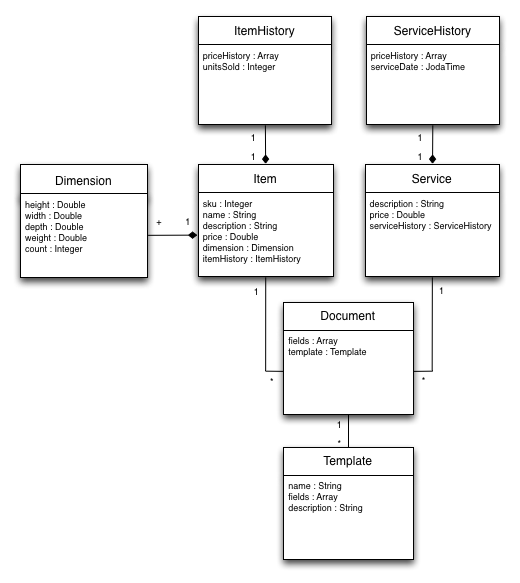
\includegraphics[width=6.5in]{../../UML/eccms-DomainObject Class Diagram.png}
\caption{Top-Level Class Diagram}
\label{server-class}
\end{figure}

\begin{figure}[H]
\centering
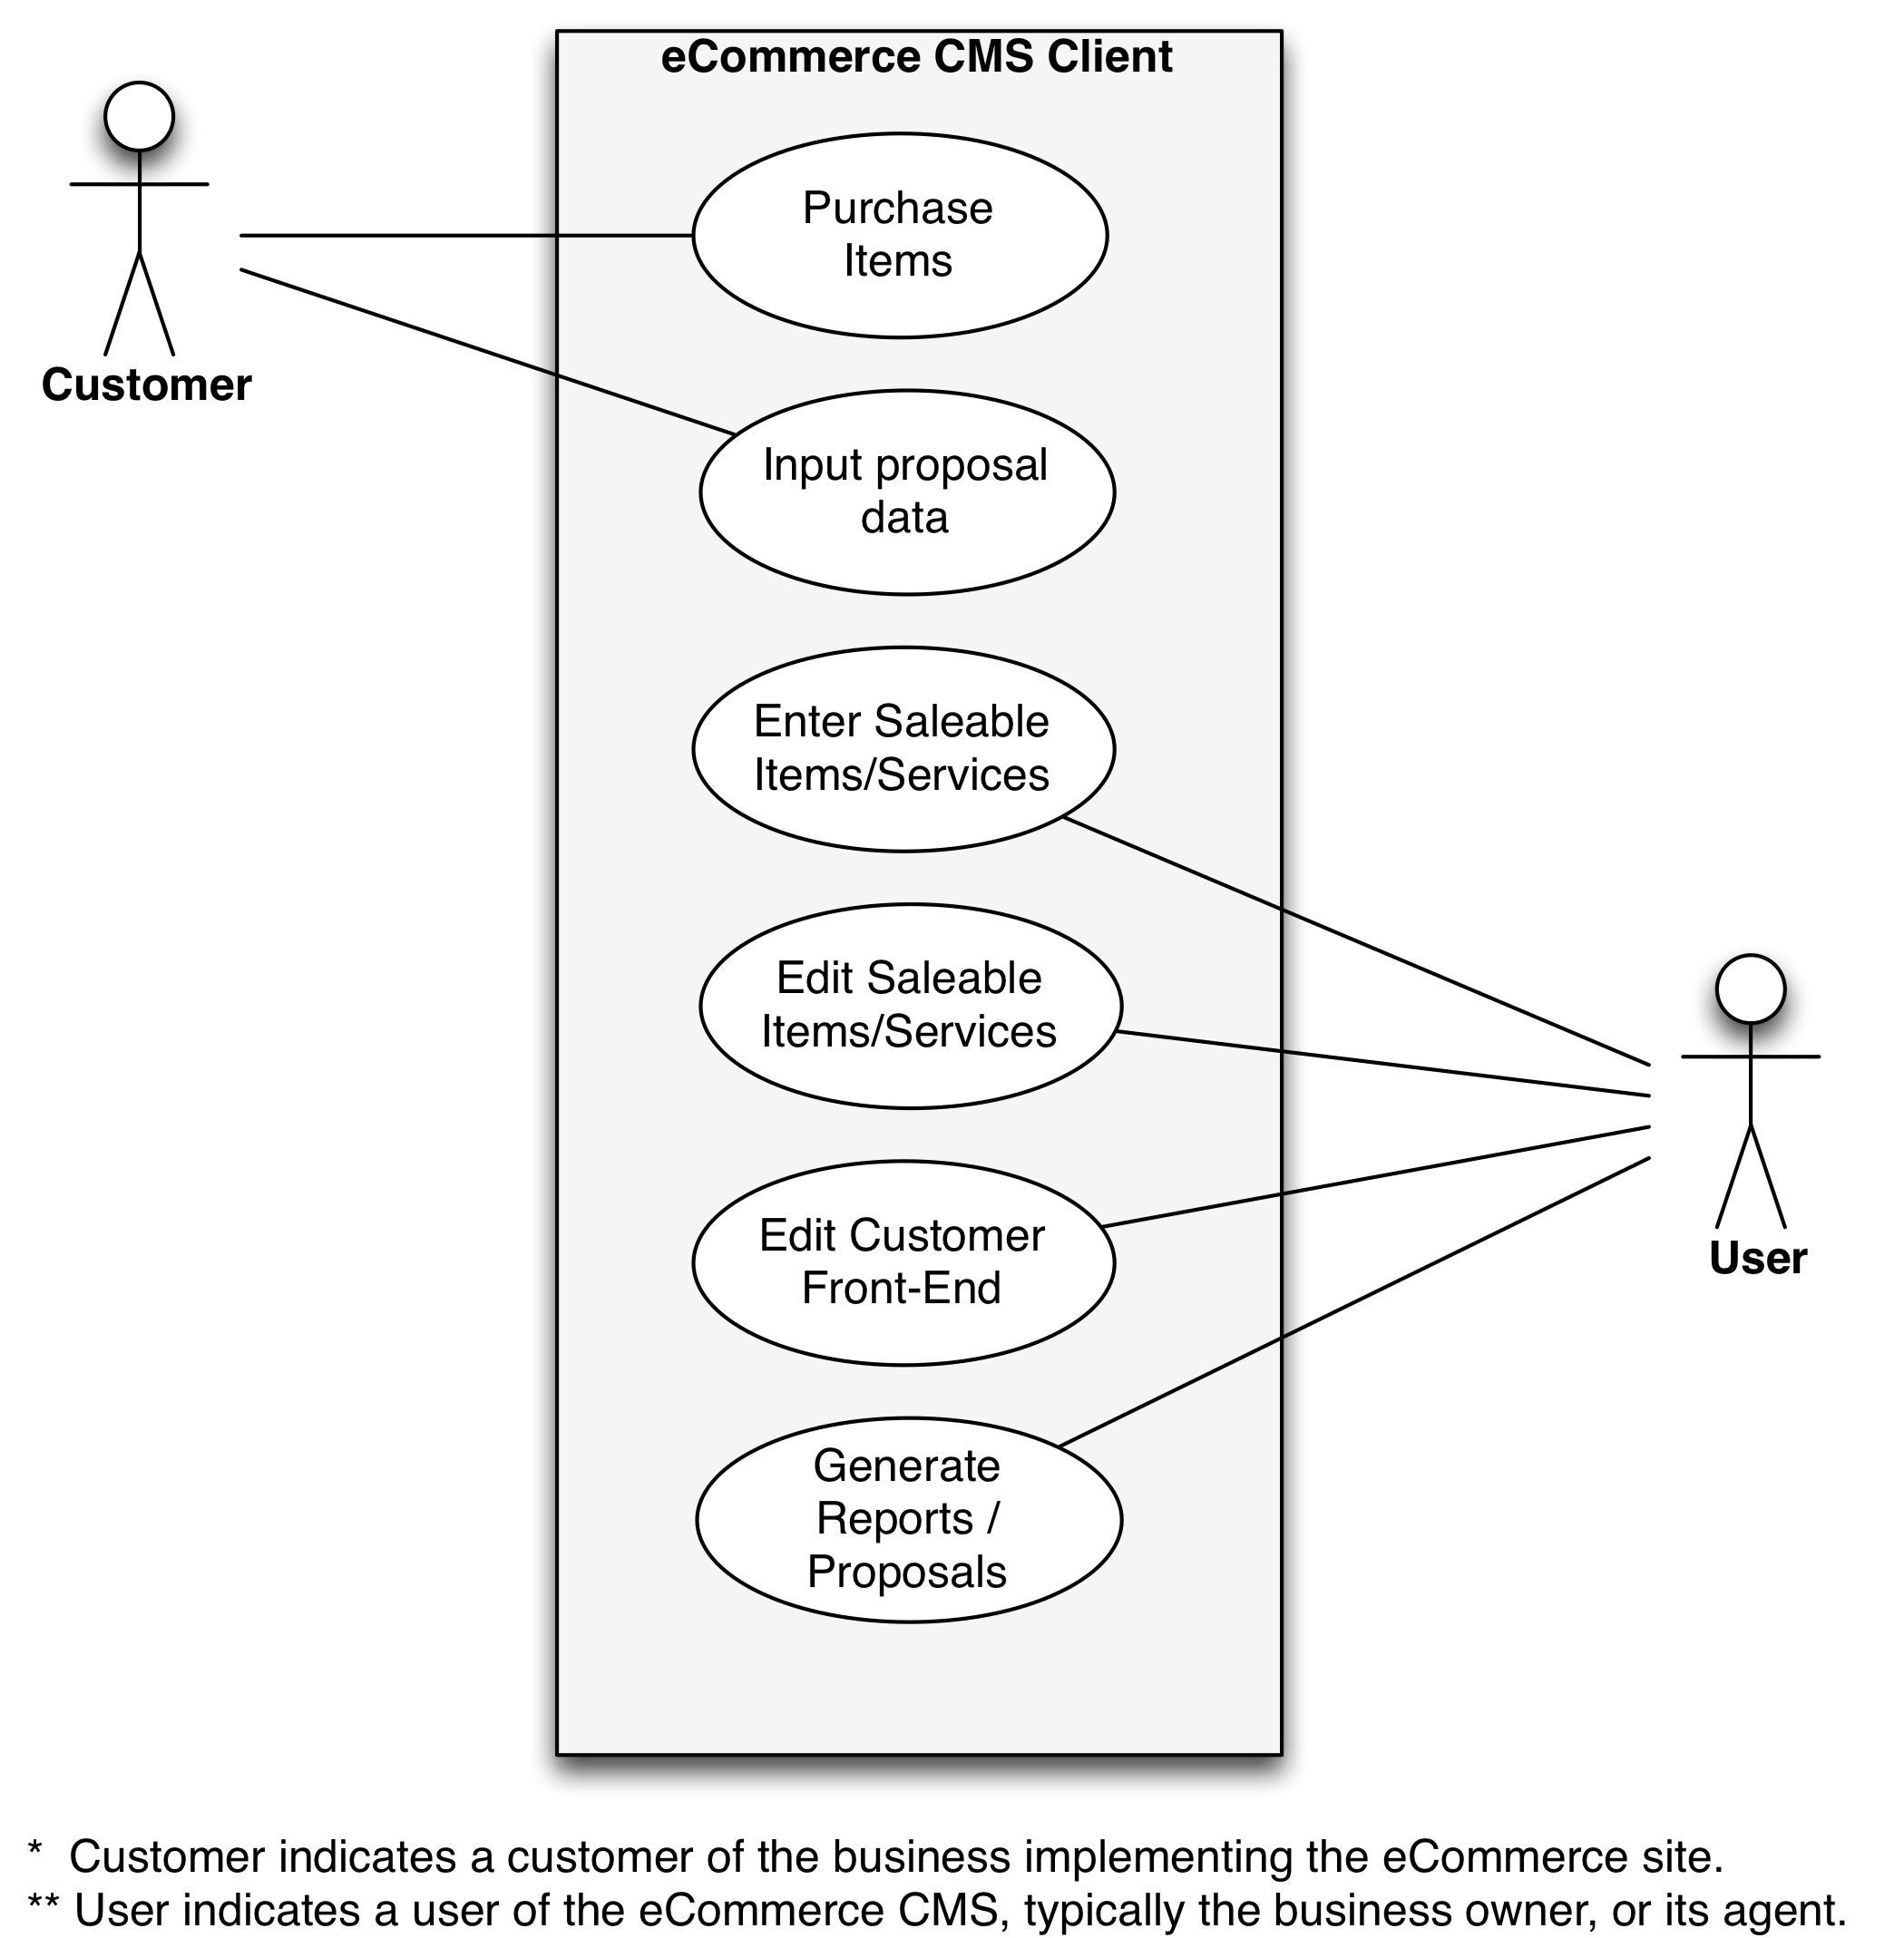
\includegraphics[width=4.5in]{../../UML/eccms-Use Case (Client) Diagram.png}
\caption{Use-Case Diagram for Client}
\label{client-usecase}
\end{figure}

\begin{figure}[H]
\centering
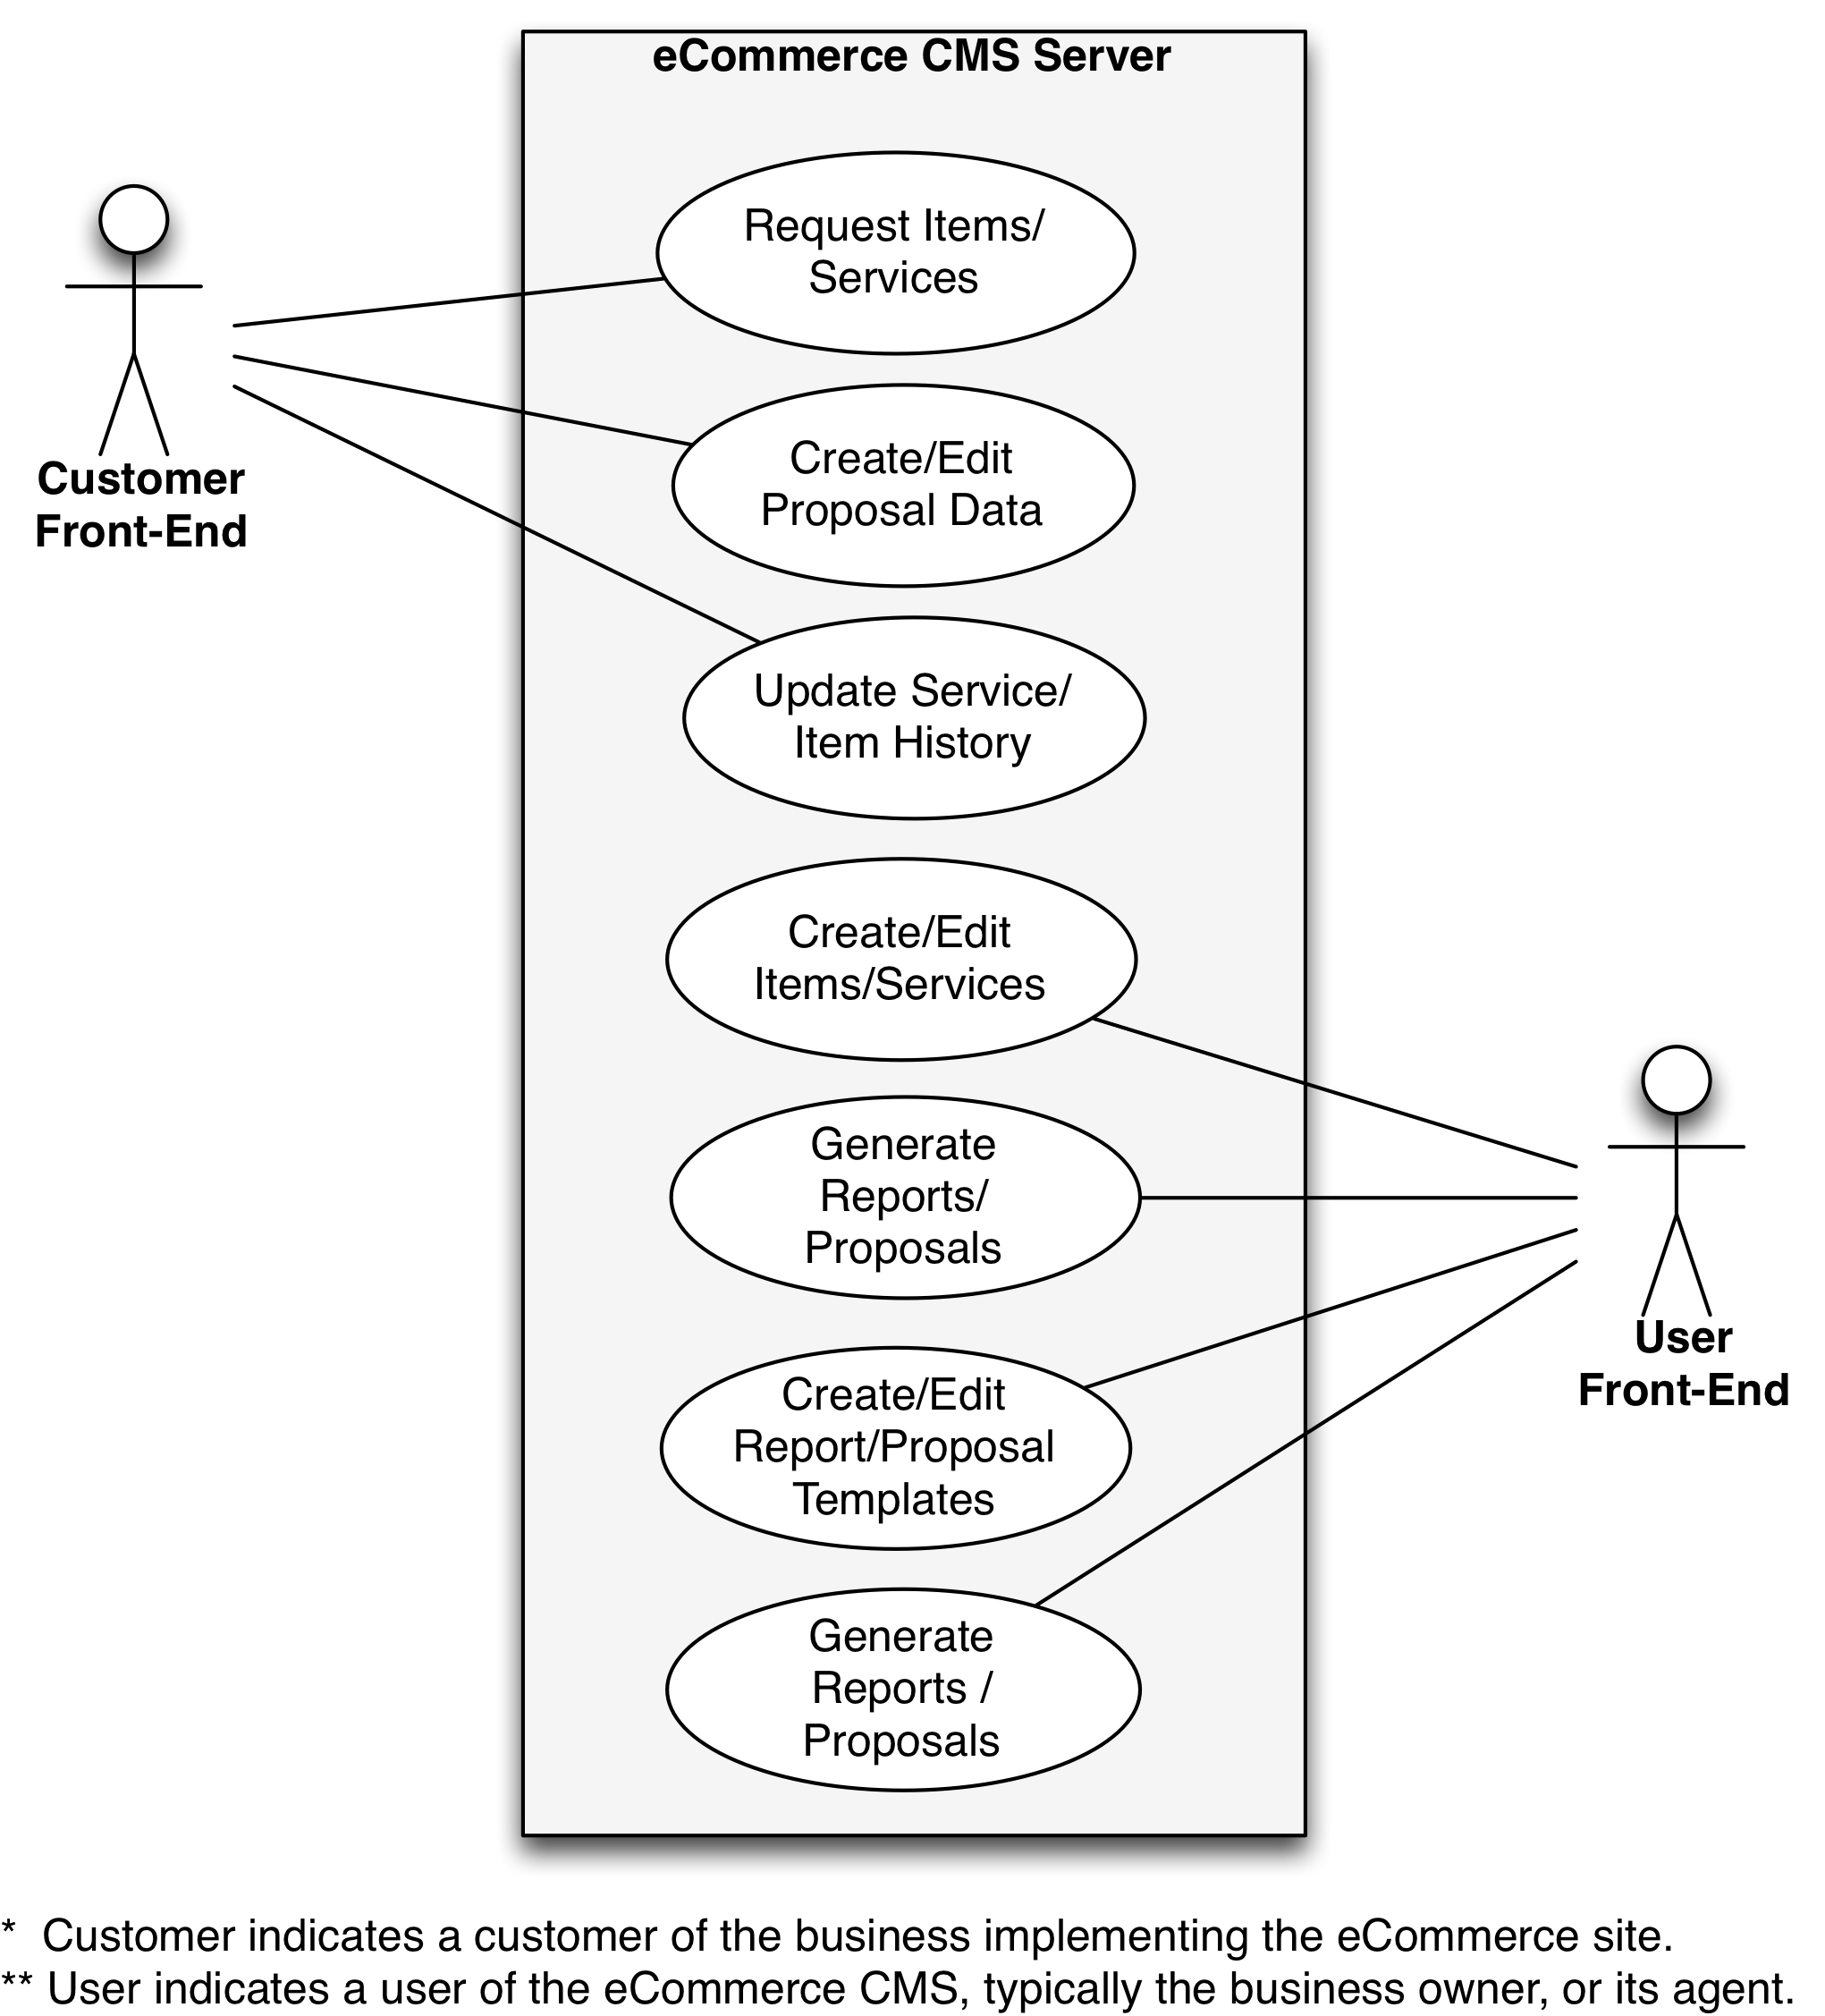
\includegraphics[width=4.5in]{../../UML/eccms-Use Case (Server) Diagram.png}
\caption{Use-Case Diagram for Server}
\label{server-usecase}
\end{figure}


\begin{figure}[H]
\centering
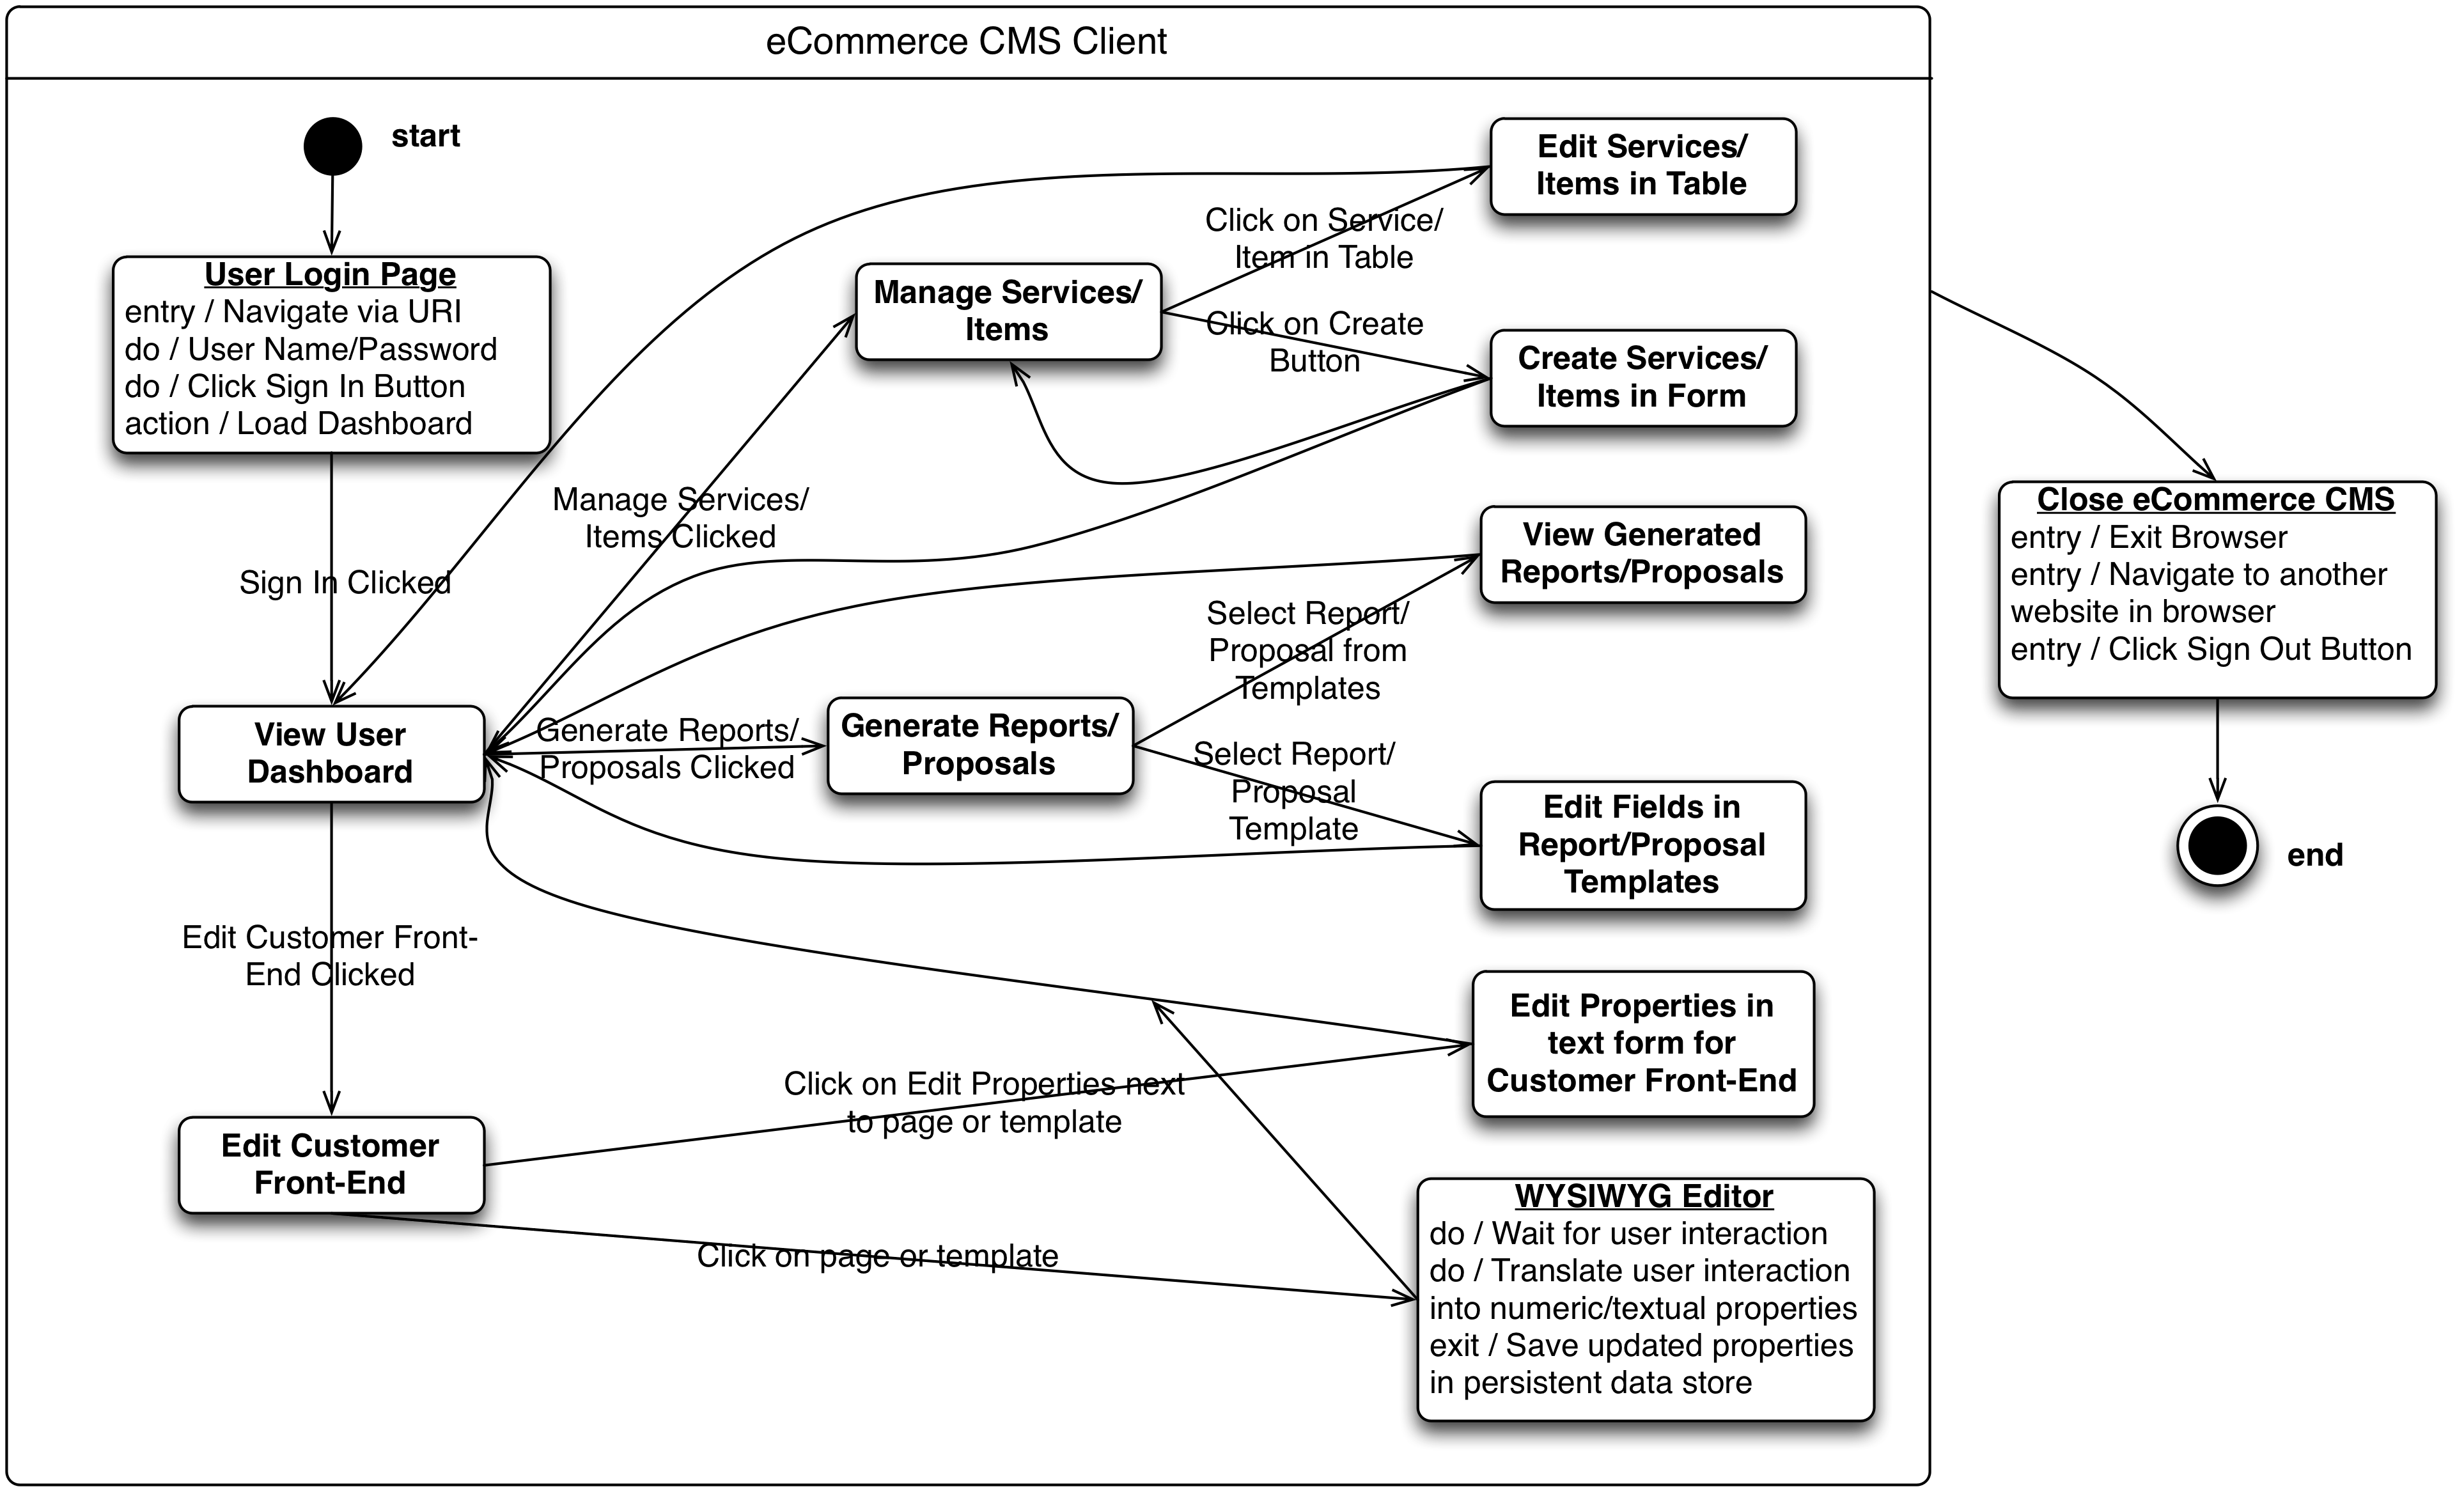
\includegraphics[width=6.5in]{../../UML/eccms-State (Client) Diagram.png}
\caption{State Diagram for Client}
\label{client-state}
\end{figure}

\begin{figure}[H]
\centering
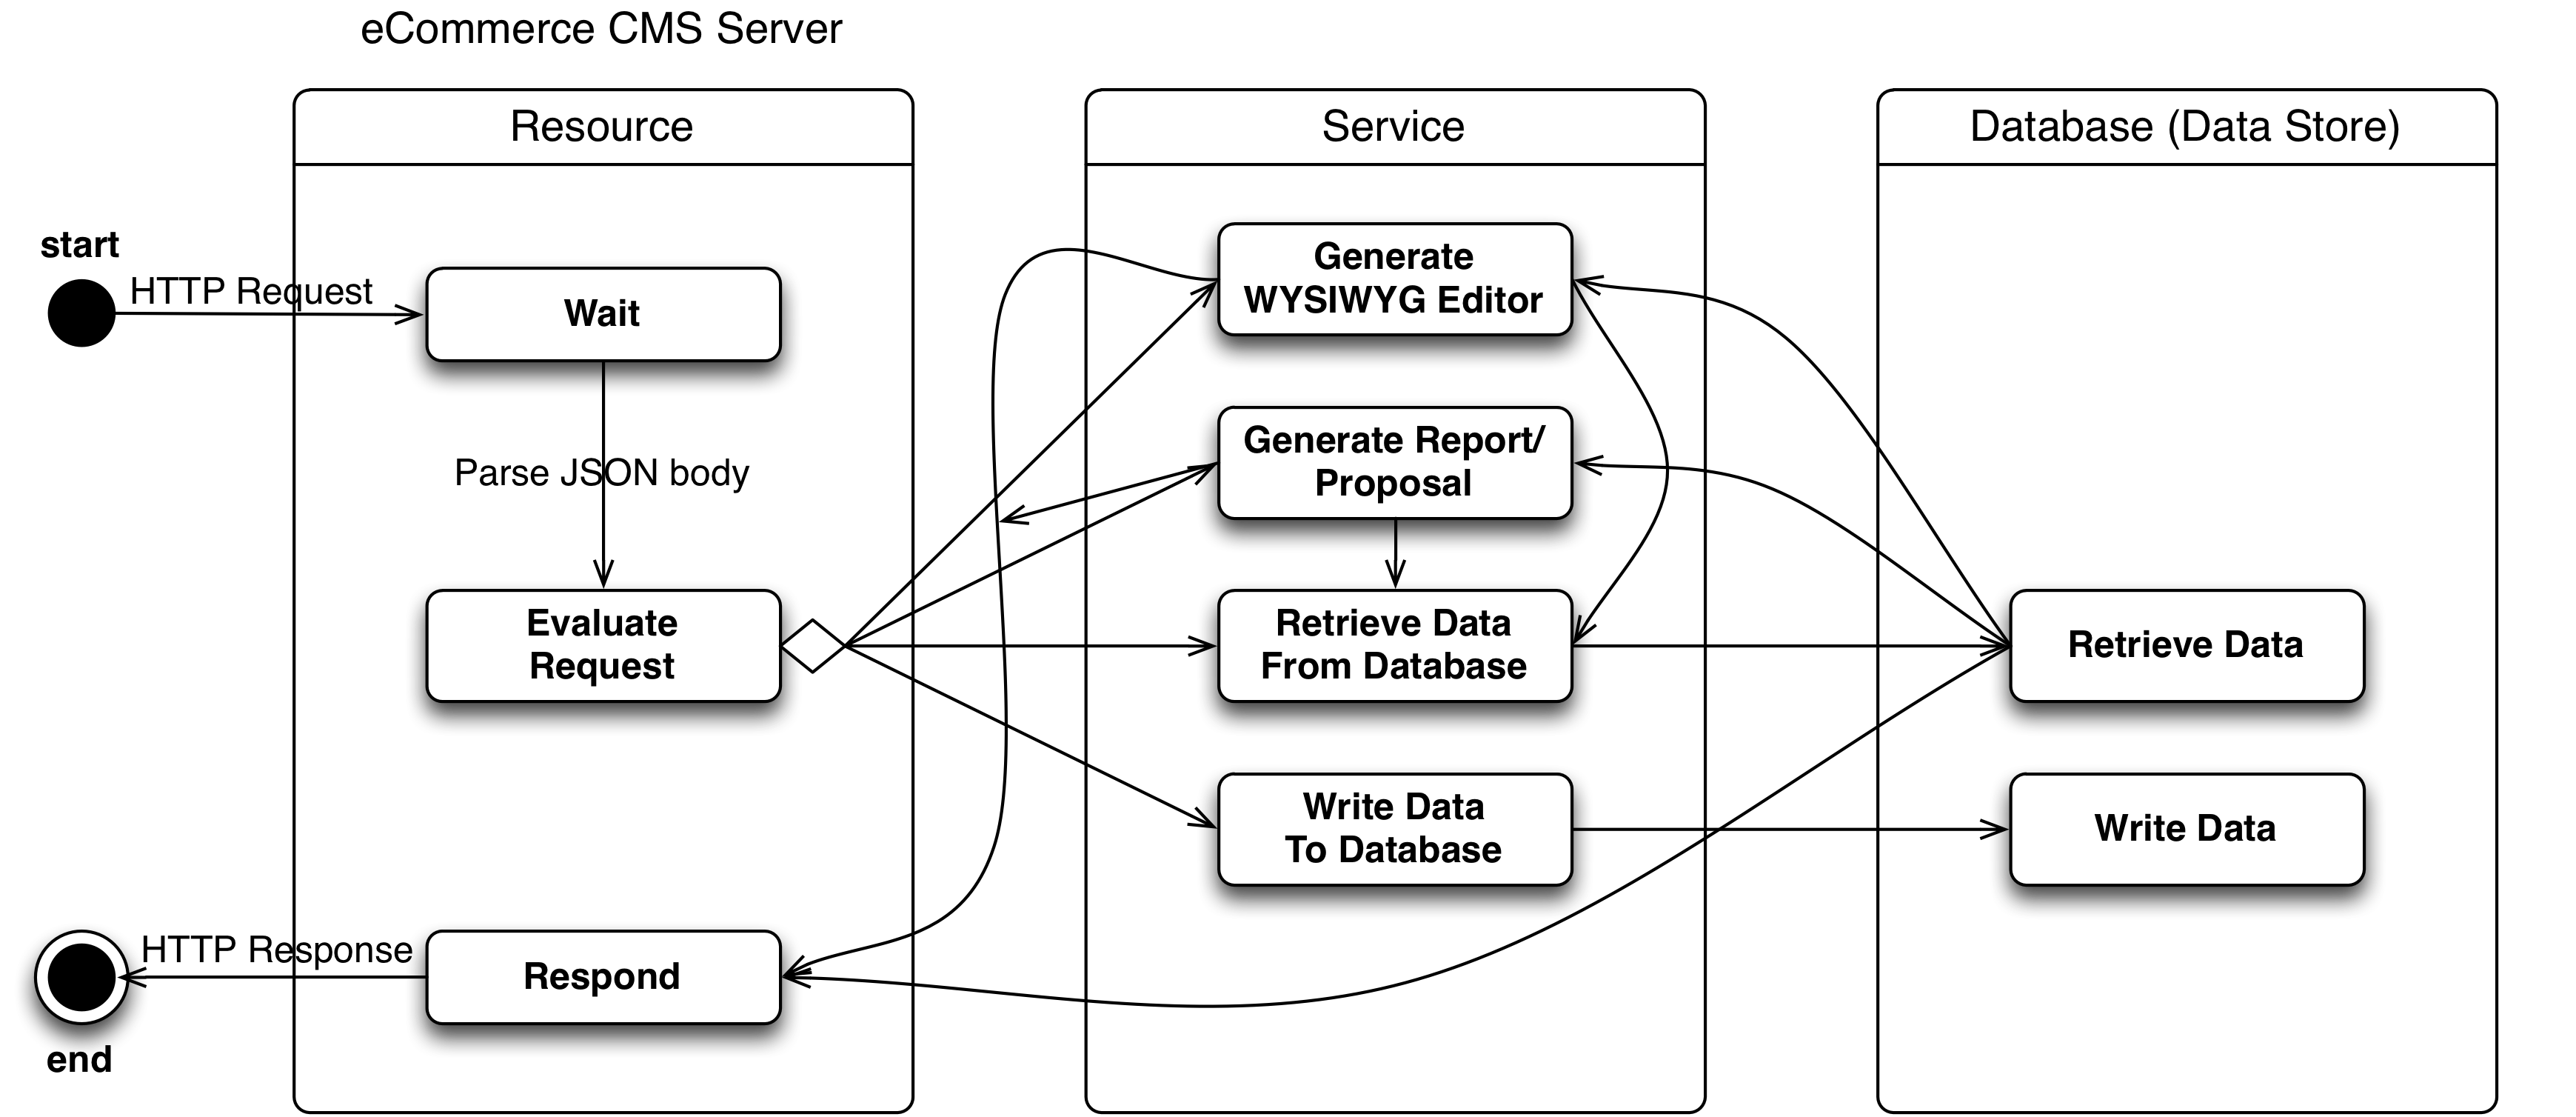
\includegraphics[width=6.5in]{../../UML/eccms-State (Server) Diagram.png}
\caption{State Diagram for Server}
\label{server-state}
\end{figure}

% In addition to the text in the previous sections, at least three UML diagrams
% of the system must be included. These several diagrams must be of several
% different types; for example, there should be a Use Case diagram of your
% system, a top-level class diagram showing the classes and the interfaces and
% their relationships to each other, a component and/or deployment diagram
% showing how the parts communicate with each other and with any external
% software or other entities, and perhaps even a swim lane diagram showing
% how your system operates at an architectural level.

\pagebreak
\subsection{CSC and CSU Descriptions}

The eCommerce CMS application is the Computer Software Configuration Item
(CSCI) and consists of three major Computer Software Components (CSC).  The
CSCI is broken down into the back-end CSC, the user front-end CSC, and the
customer front-end CSC.  Each respective CSC can further be broken down to
several Computer Software Units (CSU).  This document will specify some of the
CSU's that are intended, as listed in table~\ref{software-hierarchy}.

\begin{table}[H]
    \begin{tabular}{|c|l|p{7.5cm}|}\hline
        CSCI & CSC & CSU \\\hline\hline
        \multirow{12}{*}{eCommerce CMS}
         & Back-End & Persistent Data Store \\\cline{2-3}
         & Back-End & Report/Proposal Generator \\\cline{2-3}
         & Back-End & Front-End Generator \\\cline{2-3}
         & Back-End & Transaction Processor \\\cline{2-3}
         & User Front-End & Visual Web Page Editor \\\cline{2-3}
         & User Front-End & Web Page Template Editor \\\cline{2-3}
         & User Front-End & Inventory Input/Edit Form \\\cline{2-3}
         & User Front-End & Report/Proposal Requestor \\\cline{2-3}
         & Customer Front-End & Proposal Specification Form \\\cline{2-3}
         & Customer Front-End & Web Store \\\cline{2-3}
         & Customer Front-End & Purchasing/Transaction System \\\hline
    \end{tabular}
    \caption{CSCI, CSC, and CSU Hierarchy}
    \label{software-hierarchy}
\end{table}

% This section begins the detailed design section of the document. You begin by
% describing the Computer Software Components (CSC) and Computer Software
% Units (CSU) which comprise your application. Your application itself is a
% Computer Software Configuration Item (CSCI), which is composed of multiple
% CSCs, each of which comprises multiple CSUs. For an individual project, the
% CSUs can be your classes and interfaces. Their groupings then become the
% CSCs. Each of the CSCs must have a name, which needs to be descriptive of
% the functionality of that group of CSUs (modules, class files, interfaces,
% whatever). Each of these CSUs will be described in detail in the subsequent
% sub-sections of the document.

% An example of this might be if you are using the Model-View-Controller
% paradigm. Say your project is called the "Barbecue" project. The Model
% segment would have several classes, each of which is a CSU; collectively,
% they are the "Barbecue Model CSC". The same will follow for the other two
% CSCs, and collectively all the CSCs are called the "Barbeque CSCI".

\subsubsection{Class Descriptions}
\label{cd}

The CSU's that correspond to the back-end architecture all have corresponding
class files.  However, not all JavaScript CSU's may have class files because
JavaScript does not use classes.

\begin{enumerate}
    \item[~\ref{cd}.1 ] \emph{Back-End - Persistent Data Store}\br\\
        The persistent data store primarily consists of data-access objects (daos)
        which correspond to equivalent domain object classes.  Because these data
        access objects pertain to various functionality, these classes will be
        repeated in other sections.  The classes are as follows:
        \begin{itemize}
            \item ItemDao.java
            \item ServiceDao.java
            \item DocTemplateDao.java
            \item DocumentDao.java
            \item CustomerSiteDao.java
            \item WebTemplate.java
        \end{itemize}
    \item[~\ref{cd}.2 ] \emph{Back-End - Report/Proposal Generator}\br\\
        The Report/Proposal Generator consists of a resource file to handle HTTP
        requests, a service file to interface with the database access objects,
        a database access object to interface with the persistent data store,
        and domain objects to represent the report and proposal as a Java class.
        \begin{itemize}
            \item DocumentResource.java
            \item DocTemplateResource.java
            \item DocumentService.java
            \item DocTemplateService.java
            \item DocumentDao.java
            \item DocTemplateDao.java
            \item Document.java
            \item DocTemplate.java
        \end{itemize}
    \item[~\ref{cd}.3 ] \emph{Back-End - Front-End Generator}\br\\
        The Front-End Generator consists of a resource file to handle HTTP requests,
        a service file to interface with the database access objects, a database
        access object to interface with the persistent data store,
        domain objects to represent the customer website and templates, an interface
        for websites as a Java class, and utility classes to convert Java objects
        into HTML, CSS, and JavaScript files.
        \begin{itemize}
            \item SiteGeneratorResource.java
            \item SiteGeneratorService.java
            \item SiteGeneratorDao.java
            \item Website.java (interface)
            \item CustomerSite.java
            \item WebTemplate.java
            \item Element.java
            \item HtmlCompiler.java
            \item CssCompiler.java
        \end{itemize}
    \item[~\ref{cd}.4 ] \emph{Back-End - Transaction Processor}\br\\
        Transaction processing is handled by the Item and Service objects
        independently, and does not require additional a specific class dedicated
        to processing transactions.  The Item and Service objects will require
        resource classes to handle HTTP requests and will interface with their
        respective data access objects with service classes.
        \begin{itemize}
            \item Item.java
            \item Service.java
            \item ItemService.java
            \item ServiceService.java
            \item ItemDao.java
            \item ServiceDao.java
        \end{itemize}
    \item[~\ref{cd}.5 ] \emph{User Front-End - Visual Web Page Editor}\br\\
        The Visual Web Page Editor handles events by a JavaScript file that
        translates visual changes into numeric and textual properties to be
        transmitted to the web service.
        \begin{itemize}
            \item wysiwyg.js
        \end{itemize}
    \item[~\ref{cd}.6 ] \emph{User Front-End - Web Page Template Editor}\br\\
        The Web Page Template Editor looks like the Visual Web Page Editor, but
        the web page saved into the web service is saved as a template.  Templates
        are not accessible by a web browser outside of the web service and must be implemented
        into a web page through the Visual Web Page Editor before a customer can
        access the page.
        \begin{itemize}
            \item wysiwyg.js
        \end{itemize}
    \item[~\ref{cd}.7 ] \emph{User Front-End - Inventory Input/Edit Form}\br\\
        The Inventory Input/Edit Form will have a JavaScript file to listen for
        events and communicate with the web service.
        \begin{itemize}
            \item ims.js
        \end{itemize}
    \item[~\ref{cd}.8 ] \emph{User Front-End - Report/Proposal Requestor}\br\\
        The Report/Proposal Requestor will only have a JavaScript file to
        communicate with the web service and present a document to the user.
        \begin{itemize}
            \item docRequest.js
        \end{itemize}
    \item[~\ref{cd}.9 ] \emph{Customer Front-End - Proposal Specification Form}\br\\
        The Proposal Specification Form will have a JavaScript file to submit
        form data to the web service.
        \begin{itemize}
            \item proposalForm.js
        \end{itemize}
    \item[~\ref{cd}.10 ] \emph{Customer Front-End - Web Store}\br\\
        The Web Store will have JavaScript files to handle adding or removing
        items from the shopping cart and to retrieve items/services from the
        web service and display them on a webpage.
        \begin{itemize}
            \item shoppingCart.js
            \item store.js
        \end{itemize}
    \item[~\ref{cd}.11 ] \emph{Customer Front-End - Purchasing/Transaction System}\br\\
        The Purchasing/Transaction System has a file to communicate with the
        web service.
        \begin{itemize}
            \item checkout.js
        \end{itemize}
\end{enumerate}

% This section, and its sub-sections, describe the classes in each of the CSUs
% of the project. Each CSU must have at least one class, but there may be more.
% For these sections, you must include detailed descriptions, i.e., each class
% description contains a list of the fields for that class (with explanations
% of each field) and a separate list of the methods for that class (again with
% explanations). The main section, 6.3.1, should be some type of introductory
% paragraph such as "The following sections provide the details of all classes
% used in the <fill in the blank> application." There will be one subsection
% for each of the classes, numbered 6.3.1.1 through 6.3.1.<n>, where <n> is
% the number of classes in the project. The class descriptions should generally
% be ordered from the smallest class to the largest class so the larger classes
% can be understood at a more detailed level. Each class definition subsection
% must include a brief description of why this class is included (or of what
% its operation does for the project).

\subsubsection{Detailed Interface Descriptions}
\label{did}

The back-end classes will not directly interact with the user or customer.  The
back-end is only accessed through the web service by HTTP requests.  The following
HTTP requests may be made:

\begin{table}[H]
    \centering
    \begin{tabular}{|l|p{4.5cm}|l|}\hline
        Endpoint & Query Parameters & Description\\\hline\hline
         GET /items & page, pagesize, price, name, description, sku & Search for items. \\\hline
         GET /items/:id & -- & Get item details. \\\hline
         POST /items & -- & Create item. \\\hline
         PUT /items/:id & -- & Update item details. \\\hline
         DELETE /items/:id & -- & Delete an item. \\\hline
         GET /services & page, pagesize, price, name, description & Search for services. \\\hline
         GET /services/:id & -- & Get service details. \\\hline
         POST /services & -- & Create a service. \\\hline
         PUT /services/:id & -- & Update service details. \\\hline
         DELETE /services/:id & -- & Delete a service. \\\hline
         GET /documents & page, pagesize, templateId, field, description & Search for documents. \\\hline
         GET /documents/:id & -- & Get document details. \\\hline
         POST /documents & -- & Create a document. \\\hline
         PUT /documents/:id & -- & Update document details. \\\hline
         DELETE /documents/:id & -- & Delete a document. \\\hline
         GET /doctemplates & page, pagesize, name, field, description & Search for doctemplates. \\\hline
         GET /doctemplates/:id & -- & Get doctemplate details. \\\hline
         POST /doctemplates & -- & Create a doctemplate. \\\hline
         PUT /doctemplates/:id & -- & Update doctemplate details. \\\hline
         DELETE /doctemplates/:id & -- & Delete a doctemplate. \\\hline
         GET /websites & page, pagesize, templateId, name, description & Search for websites. \\\hline
         GET /websites/:id & -- & Get website details. \\\hline
         POST /websites & -- & Create a website. \\\hline
         PUT /websites/:id & -- & Update website details. \\\hline
         DELETE /websites/:id & -- & Delete a website. \\\hline
         GET /webtemplatess & page, pagesize, price, name, description & Search for webtemplatess. \\\hline
         GET /webtemplatess/:id & -- & Get webtemplates details. \\\hline
         POST /webtemplatess & -- & Create a webtemplates. \\\hline
         PUT /webtemplatess/:id & -- & Update webtemplates details. \\\hline
         DELETE /webtemplatess/:id & -- & Delete a webtemplates. \\\hline
    \end{tabular}
    \caption{HTTP Request Web Service Endpoints}
    \label{endpoints}
\end{table}

\begin{enumerate}
    \item[~\ref{did}.1 ] \emph{User Front-End - Visual Web Page Editor}\br\\
    \item[~\ref{did}.2 ] \emph{User Front-End - Web Page Template Editor}\br\\
    \item[~\ref{did}.3 ] \emph{User Front-End - Inventory Input/Edit Form}\br\\
    \item[~\ref{did}.4 ] \emph{User Front-End - Report/Proposal Requestor}\br\\
    \item[~\ref{did}.5 ] \emph{Customer Front-End - Proposal Specification Form}\br\\
    \item[~\ref{did}.6 ] \emph{Customer Front-End - Web Store}\br\\
    \item[~\ref{did}.7 ] \emph{Customer Front-End - Purchasing/Transaction System}\br\\
\end{enumerate}

% TODO: talk about what reports can be generated

% This section, and its sub-sections, describe the interfaces in each of the
% CSUs of the project. Follow the same guidelines as described in the paragraphs
% above, only for interfaces rather than classes.

\subsubsection{Detailed Data Structure Descriptions}
\label{ddsd}

All database queries will be parsed into plain-old Java objects (POJOs).  The
POJOs will contain either java ArrayLists or java Stacks depending upon how
the data will have to be accessed.

% This section, and its sub-sections, describe the data structures in each of
% the CSUs of the project. Data structure details consist of things like the
% in-depth description of message packets, database query results, and any
% other non-class and non-interface data structures. For example, if you are
% implementing a form of a doubly-linked list or a queue, include a description
% of the structure, for what purpose it will be used, and any methods or
% operations in which it will be involved. Follow the same guidelines as
% described in the two preceding paragraphs.

\subsubsection{Detailed Design Diagrams}
\label{ddd}

% In this section, you must include all detailed diagrams for all facets of the
% project. This means you will need to have detailed use case diagrams,
% package diagrams, class diagrams, and either activity, swim lane, sequence,
% or state diagrams. You need to show in diagram form the actual workings of
% the project. The intent of sections 6.3 and 6.4 (and if needed, 6.5) is to
% provide a start for the code phase of the project. You should be able to
% start coding directly from these descriptions, and should see the interplay
% of all parts from the diagrams. Be sure to use correct UML for all diagrams.
% You can use whatever tool you like to draw the UML, whether it be a CASE tool
% like Poseidon or a simple drawing tool like Impress. Just make sure the
% diagrams are legible, meaningful, and drawn as correctly as possible.

\pagebreak
\subsection{Database Design and Description}

\subsubsection{Database Design ER Diagram}
\label{dded}

\subsubsection{Database Access}
\label{da}

\subsubsection{Database Security}
\label{ds}

% These sections are all lumped together, since they may be optional. If you
% have no database in your project, simply include section 6.4, and insert a
% paragraph stating there is no database involved in the project. If there is
% a database as part of your application, then you must describe it. Include a
% complete and correct UML Entity-Relationship diagram in section 6.4.1, a
% paragraph or two about how the database will be accessed in 6.4.2, and another
% paragraph or two about how you are implementing database security in 6.4.3.
% Make this section consistent with the other sections of the document.

\end{document}